\documentclass[a4paper,12pt]{article}
\usepackage{fancyhdr}
\usepackage{graphicx}
\usepackage[utf8]{inputenc}


\title{Design Analysis}
\author{Group Project 3 - Group 2}
\date{March 21 2008}

\begin{document}
\maketitle
\newpage
\tableofcontents
\newpage



\section{Introduction}
The diagram includes the classes discovered during analysis, plus some additional classes discovered during design.


\section{Class diagram}
\begin{figure}[htbp]
\begin{center}
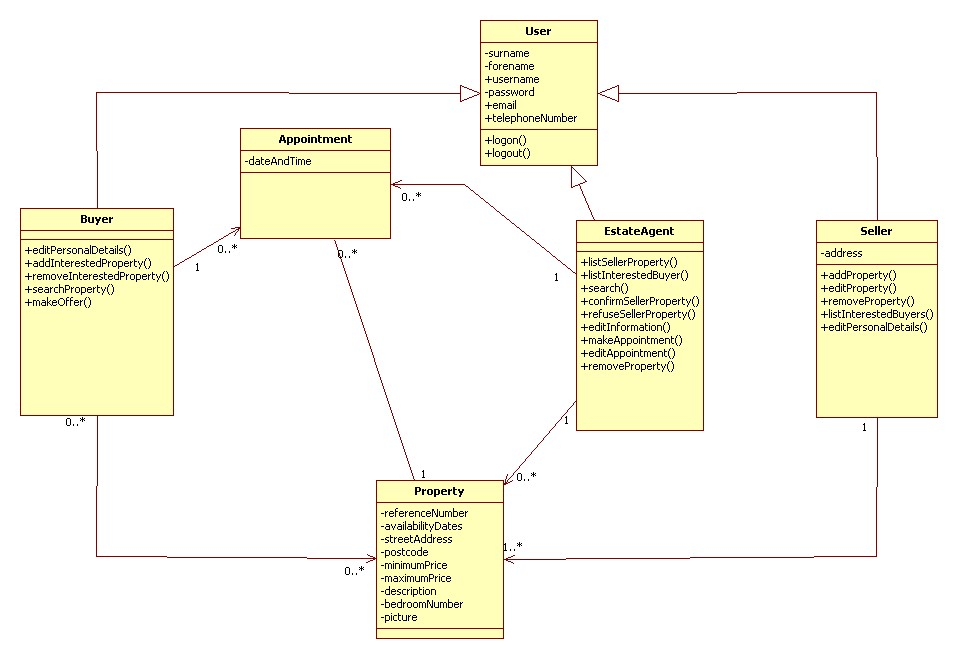
\includegraphics[width=\linewidth]{pics/classDiagram.jpg}
\end{center}
\caption{\footnotesize Class Diagram of Napier Estate Agency}
\end{figure}
\subsection {Model classes}

\subsubsection{EstateAgent class}

\subsubsection{Buyer class}

\subsubsection{Seller class}

\subsubsection{User class}
The Seller class , the Buyer class and the EstateAgent class has common attributes: surname, forename, username, password and email.
This will guide us that a common class can be introduced.
This will be a good time to make an inheritance.
Parent class will be User and will hold common attributes for Seller, Buyer and EstateAgent, and these operations: logon() and logout().
The Seller, the Buyer and the EstateAgent classes (children of this class) will have their respective operations.

\subsubsection{Property class}

\subsubsection{Appointment class}

\subsection {Controler classes}

\end{document}
